\documentclass[10pt,letterpaper]{article}
\usepackage{tools}
\usepackage{enumitem}
%\settextfont{B Nazanin}
\usepackage{lipsum}
\setlength{\parskip}{3mm}
\setlength{\parindent}{0mm}
\newcommand{\wid}{0.49\textwidth}
\newcommand{\widone}{60mm}
\begin{document}
\Large
\begin{center}
In the name of beauty

6th problem set of ComNet course
\hl
\end{center}
Q1)
\begin{enumerate}[label=\alph*-]
\item
False. In this case, the sender sends a byte to retreive the newest receiver state.
\item
False. Only the first two packets have the SYN bit equal to 1. Afterwards, the connection is setup and the SYN bit is 0. Also at the end of a connection, the buffers are not deallocated immediately since the yet-to-arrive packets still need to reach their destination (in TCP mode).
\item
False. This paradigm holds in network-assisted congestion control. The end-to-end congestion control is implemented only at Transport Layer.
\item
True. This is the most important tool for triggering transmission rate.
\item
True. For instance, the Tahoe version of congestion control did not include fast recovery.
\item
True based on the congestion control FSM.
\end{enumerate}

Q2)

At the end of the first time slot, two packets have been downloaded from the media and one of them is completely read to the Application Layer. Hence, we end up with a total of 1500bytes at the buffer.
\begin{enumerate}[label=\alph*-]
\item
\texttt{rwnd}=1500 bytes
\item
The receiver advertises \texttt{rwnd}=0 at the end of the 4-th time slot. The sender, having received this message, gives up sending too many bytes and suffices to 1 byte to assess the receiver's state.
\end{enumerate}

Q3)

\begin{enumerate}[label=\alph*-]
\item
1 to 6 and 23 to 26.
\item
7 to 16 and 17 to 22
\item
It is a triple duplicate ACK since the time out would reset the \texttt{cwnd} to 1.
\item
It is a time out since the \texttt{cwnd} has been reset to 1.
\item
It is equal to 32 since after this phase of transmission, the sender has entered the congestion avoidance state.
\item
$$
\texttt{ssthresh}_{18}={\texttt{cwnd}_{16}\over 2}={42\over 2}=21
$$
\item
$$
\texttt{ssthresh}_{24}={\texttt{cwnd}_{22}\over 2}={29\over 2}=14 \text{ or }15
$$
\item
For the first 6 transmission rounds, the segments numbered from $2^{n-1}$ to $2^n-1$ have been transmitted. Hence, at the end of the 6th transmission round, we have $2^6-1=63$ segments transmitted. Since \texttt{cwnd}=33 at the 7th transmission round, we have segments 64 to 97 (including) sent to the receiver.
\item
$$
\texttt{ssthresh}_{27}={\texttt{cwnd}_{26}\over2}=4
$$
$$
\texttt{cwnd}_{27}=\texttt{ssthresh}_{27}+3=7
$$
\item
TCP Tahoe does not support fast recovery and treats a three-duplicate-ACK situation just like a time out. The result is as follows:
$$
\texttt{ssthresh}_{19}={\texttt{cwnd}_{16}\over2}=21
$$
$$
\texttt{cwnd}_{19}=1\times 2\times 2=4
$$
\item
The \texttt{cwnd} is reset to 1 at round 17, hence we have 1, 2, 4, 8 and 16 segments transmitted at rounds 17 to 21 and 21 segments transmitted at round 22 due to reaching the \texttt{ssthresh}, yielding a total number of 52 segments.
\end{enumerate}

%{\huge (Figure 1 on next page)}
%
%\begin{figure}[htbp]
%\centering
%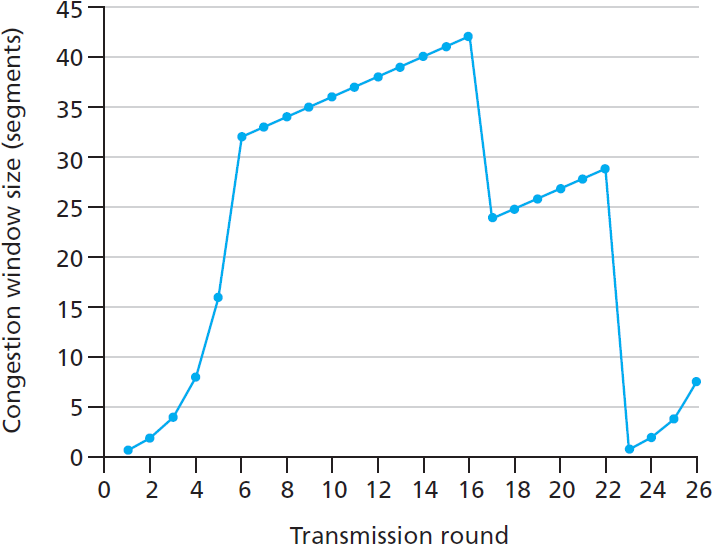
\includegraphics[width=150mm]{congestion.png}
%\caption{TCP window size as a function of time}
%\end{figure}
\end{document}